\documentclass[conference]{IEEEtran-modified}

\renewcommand{\figurename}{Figure}

\usepackage{float}
\usepackage[pdftex]{graphicx}
\usepackage[export]{adjustbox}
\graphicspath{{./figures/}}
\usepackage[sort, numbers]{natbib}
\setcitestyle{square}
\usepackage[table]{xcolor}
\usepackage{tikz}
\usepackage{amsmath}
\usepackage{listings}
\usepackage{color}
\usepackage{caption}


% Custom colors
\definecolor{navyblue}{RGB}{31,73,125}
\definecolor{burgundy}{rgb}{0.5, 0.0, 0.13}
\definecolor{lightgray}{rgb}{.6,.6,.6}
\definecolor{darkgray}{rgb}{.2,.2,.2}


\lstdefinelanguage{JavaScript}{
  keywords={typeof, new, true, false, catch, function, return, null, catch, switch, var, if, in, while, do, else, case, break},
  keywordstyle=\color{lightgray}\bfseries,
  ndkeywords={class, export, boolean, throw, implements, import, this},
  ndkeywordstyle=\color{darkgray}\bfseries,
  identifierstyle=\color{black},
  sensitive=false,
  comment=[l]{//},
  morecomment=[s]{/*}{*/},
  commentstyle=\color{lightgray}\ttfamily,
  stringstyle=\color{burgundy}\ttfamily,
  morestring=[b]',
  morestring=[b]"
}

\lstset{
   language=JavaScript,
   backgroundcolor=\color{white},
   extendedchars=true,
   basicstyle=\footnotesize\ttfamily,
   showstringspaces=false,
   showspaces=false,
   numbers=none,
   numberstyle=\footnotesize,
   numbersep=9pt,
   tabsize=2,
   breaklines=true,
   showtabs=false,
   captionpos=b
}


% Scientific notation
\providecommand{\e}[1]{\ensuremath{\times 10^{#1}}}

\begin{document}

\title{Rotation Curve Modeler \\ \Large{A Modeling and Simulating Tool for Arbitrary Galaxies}}

\author{
\IEEEauthorblockN{Robert J. Moss}
\IEEEauthorblockA{Lincoln Laboratory\\
Massachusetts Institute of Technology\\
%Department of Computer Science and Networking\\
%Wentworth Institute of Technology\\
%Boston, Massachusetts 02115\\
%mossr@wit.edu\\
Lexington, Massachusetts 02420\\
robert.moss@ll.mit.edu}
\and
\IEEEauthorblockN{Dr. James G. O'Brien}
\IEEEauthorblockA{Department of Applied Math and Sciences\\
Wentworth Institute of Technology\\
Boston, Massachusetts 02115\\
obrienj10@wit.edu}
}

\onecolumn

%\twocolumn[
%  \begin{@twocolumnfalse}
%	
%
%  \end{@twocolumnfalse}
%]

	\maketitle
    \begin{abstract}
	
	In order to best understand the current dark matter paradigm, one must have a firm understanding of the rotation curve problem, as well as the underlying theories which explain the rotation curves themselves.  Also in modern literature, many alternative gravitational theories are appearing with more frequency and potency. Although specific galaxies can be modeled in a fairly straight forward manner (depending on the assumed theory), it may not be as intuitive to compare various models on a particular galactic rotation data set.  Moreover, it can prove difficult to sift through peer-reviewed articles to collect data and parameter sets that astronomers have published on various galaxies. Here, we present potential solutions to these problems with a Rotation Curve Modeler, to model arbitrary galaxies, a Scholarly Observed Celestial Measurements database, to house all the galactic data in a central location, and a Rotation Curve Simulation, to simulate the spin of star clusters around the center of a galaxy.
	\end{abstract}
	
	
	\begin{IEEEkeywords}
	\begin{center}
	galaxy, rotation curve, modeling, simulating, general relativity, lambda cold dark matter, conformal gravity.
	\end{center}	
	\end{IEEEkeywords}
	
	
	\IEEEpeerreviewmaketitle
% Page numbers
\thispagestyle{plain}
\pagestyle{plain}

\section{Introduction}
To model the rotation of single galaxies, astrophysicists would use programs like MATLAB or Mathematica, but there doesn't exist a singular tool to expedite this process in a universal format.   More importantly, their does not exist a current singular tool which can simultaneously model galaxies across competing gravitational theories.  In this paper, we introduce The Rotation Curve Modeler (RoCM) to serve as this tool to model the rotation of star clusters around the center of a galaxy. The tool will also aid theorists working to study alternate theories to dark matter, by its ability to test all existing galactic models against the observational data for the specified galaxy simultaneously. With observable data from astronomers as the input, any arbitrary galaxy can be imported into the tool. Tho RoCM tool is also designed to be dynamic, and enable users to import their own galactic models to test against existing theories.  Perhaps the most useful and unique features of RoCM, are its parameter value sliders, which allow users to control free fitting parameters within the models with real-time visual feedback in the generated graph. This way, each model can be finely tuned to the data, in a real time method while still yielding all of the same statistical measurements of single run galaxy modelers. The modeler makes no bias against the physicality of the specific model, but can thus be used as a full range exploration of the parameter space in question.  RoCM is designed to be a stand alone program which can import data sets from astronomical papers, but has also been designed to work with the second phase of the project, the Scholarly Observed Celestial Measurements database. As can be seen in \cite{impact} for even a sample of 11 galaxies, parameters and data had to be pulled from over 20 different references.  

%%%



\section{The Rotation Curve Problem}

%\subsection{The Rotation Curve Problem}
The physicist Fritz Zwicky working in 1933 for the California Institute of Technology observed the red shift of star clusters within galaxies and stated that the expected velocity was entirely off pace with prediction. The proposed theory was that a matter invisible to the eye -- dark matter -- was in need to account for missing mass that would otherwise hold the clusters together \cite{zwicky}. He proposed that there were ``faint galaxies and diffused gas" that filled in this void \cite{zwicky}. It was later confirmed that such gas was indeed within the galaxy, and as telescopes moved from optical to radio telescopes, the fidelity was high when measuring the amount of gas thanks to the success of spectroscopy.  Although we can now account for this ``missing mass'', many years of evidence has shown that the amount from gas was no where near the volume that was missing in the overall observation. 

Later in the 1970's, Vera Rubin and her colleague, Kent Ford, worked with a new spectrograph that could observe the rotation velocity of spiral-galaxies with incredible accuracy; in both the optical and radio bands \cite{rubin1980}. Upon further research, they concluded that the stars were moving with a uniform velocity around the center of the galaxies, rather than gradually declining in velocity further out (as predicted by general relativity).  Moreover, as their observations advanced, the uniform velocity seemed to trend across all sizes and shapes of galaxies, which would rule out effects of star formation and or galactic evolution. Their findings brought along much speculation.  Since at its heart, the predicted velocity $v$ for the star clusters is a function of only two observational parameters, the distance from the galactic center and the mass of the galaxy. It was realized that if there was invisible mass in the outer regions of galaxies, the prediction and data could be reconciled. This missing factor that increased the predicted velocity is highly thought to be dark matter, yet as can be seen in current literature, with the appearance of many competing alternative gravitational theories, the true answer still remains a mystery.
The rotation curve problem has been around for almost a century. Since it's origin, theories have surfaced that claim to solve it. RoCM was built for the purpose of comparing the theories that attempt to solve the ``missing mass'' problem in galaxy rotation curves.

\section{Parameter Fitting for Models in RoCM}
Each galaxy has a common set of parameters that may be used as model inputs: 
\begin{table}[h]
	\centering
	\normalsize
	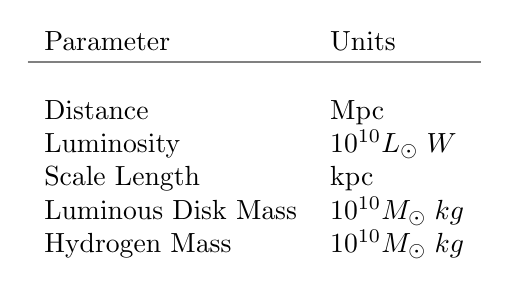
\begin{tikzpicture}
	\node[fill=white,inner sep=0pt] 
	{\rowcolors{1}{white}{white}
		\begin{tabular}{ l l }
		Parameter & Units \\
		\arrayrulecolor{gray}\hline
		\arrayrulecolor{gray}\hline
		&\\
		Distance & Mpc \\
		Luminosity & $10^{10} L_{\odot} \; W$\\
		Scale Length & kpc\\
		Luminous Disk Mass & $10^{10} M_{\odot} \; kg$\\
		Hydrogen Mass & $10^{10} M_{\odot} \; kg$\\
		
		\end{tabular}
	};
	\end{tikzpicture}
\end{table}

A quick summary is as follows: \emph{Distance} is the assumed distance from the observed galaxy to us here on earth making the measurements.  \emph{Luminosity} is the assumed luminosity of the observed galaxy which is distance dependent.  \emph{Scale Length} is the observed luminosity profile exponential falloff, assuming that galactic density is given by 
\begin{equation}
\Sigma(R)=\Sigma_0e^{\frac{-R}{R_0}}\\
\end{equation}
where {$R_0$} is the scale length, and {$\Sigma_0$} is the central density and is thus ultimately related to the later described parameter {$N^*$}.  \emph{Luminous Disk Mass} is the amount of luminous matter in the galaxy, and \emph{Hydrogen Mass} is the assumed mass of the hydrogen gas present in the galaxy, which like many of the others above, also scales with the assumed distance.
Due to the nature of the measurements, astronomers always provide a range for observed parameters. Each galaxy has an accepted range for the number of stars, $N^*$, which is calculated as a ratio of the luminous disk mass over solar mass,
\begin{equation}
N^* = \frac{M_{disk}}{M_{\odot}}.
\end{equation}

\subsection{General Relativity Prediction}

Referenced from \cite{mannheim}, the normalization free parameter, $N^*$, scale length, $R_0$, Schwarzschild radius, $\beta^*$, and the speed of light, $c$, are used in general relativity to model a galaxy's rotation velocity as a function of galactocentric distance, $R$, in the form
\begin{equation}
v_{GR}(R) = \sqrt{\frac{N^*\beta^*c^2R^2}{2R^3_0}F_b}
\end{equation}
where the bessel functions $I_0$, $I_1$, $K_0$, and $K_1$ are used to formulate the curve
\begin{equation}
F_b = \left[I_0\left(\frac{R}{2R_0}\right)K_0\left(\frac{R}{2R_0}\right)-I_1\left(\frac{R}{2R_0}\right)K_1\left(\frac{R}{2R_0}\right)\right].
\end{equation}
It is assumed that each parameter is fixed (other than the input $R$). But since these fixed parameters have an accepted range, it's difficult to alter them and see the behavior of the model in a single run program.   


\subsection{Lambda Cold Dark Matter}
An issue when modeling galaxies is how to best adjust a free parameter like $N^*$. Some models have more free parameters than others, all dictated by the theory. The $\Lambda CDM$ theory states that each galaxy has two unobservable parameters, namely the spherical dark matter density, $\sigma_0$, and the dark matter halo radius, $r_0$. As described by \cite{mannheim}, the $\Lambda CDM$ rotation velocity contribution
\begin{equation}
v_{dark}(R) = \sqrt{4\pi\beta^*c^2\sigma_0\left[1-\frac{r_0}{R}\text{arctan}\left(\frac{R}{r_0}\right)\right]}
\end{equation}
is summed with the general relativity contribution to produce a total dark matter rotation velocity of 
\begin{equation}
v_{total}(R) = \sqrt{v_{GR}^2 + v_{dark}^2}.
\end{equation}

In order for $\Lambda CDM$ to work, $\sigma_0$ and $r_0$ have to be fit to the data using a $\chi^2$ test against $v_{total}$. The two free parameters effectively shape the modeled rotation curve to make it precisely fit the data. The problem with parameter fitting is that it's time consuming and can be tough to initialize minimum and maximum ranges without any empirical evidence to suggest a initial value range. To expedite this process, RoCM provides parameter fitting sliders to quickly and visually test each parameter value in the models, thus allowing the user to have a true interaction with the model on a real time basis.

\subsection{Alternative Gravitational Models}
Since one of the goals of RoCM is to compare models of rotation curves on the fly, we shall without loss of generality use the alternative gravitational theory known as Conformal Gravity to illustrate the scope of RoCM.  Starting with the principle equations of GR, conformal gravity deems to replace GR, but allows it to stay true under certain scales \cite{mannheim}. 
Not intended to solve the rotation curve problem, conformal gravity seeks to formulate an equally good theory of gravity that is more inclusive than GR. Conformal gravity retains a metric theory of gravity but also includes the feature of conformal invariance. In short, CG require three additional terms to the GR equation to be appended, $\gamma^*$, $\gamma_0$, and $\kappa$ \cite{mannheim}. These constants include missing feasible physical parameters that Einstein didn't need in order for him to model the solar system. Now that physicists need to model objects at a greater scale, the parameters that were initially scrapped from the theory of general relativity have now been added back in.
 As described by \cite{mannheim}, the final rotation velocity function derived from conformal gravity is given by
\begin{equation}
v_{CG}(R) = \sqrt{\genfrac{}{}{0pt}{}{v_{GR}^2+\frac{N^*\gamma^*c^2R^2}{2R_0}I_1\left(\frac{R}{2R_0}\right)K_1\left(\frac{R}{2R_0}\right)}{+\frac{\gamma_0c^2R}{2}-\kappa c^2R}}
\end{equation}
where the constants are
\begin{equation*}
\begin{split}
\gamma^*=5.42\e{-41} {\rm cm}^{-1}, \\ 
\gamma_0=3.06\e{-30} {\rm cm}^{-1}, \\ 
\text{and}\; \kappa=9.54\e{-54}~{\rm cm}^{-2}.
\end{split}
\end{equation*} 

These small terms exist only at certain scales. This allows conformal gravity to scale down to the solar system, making the three additional terms negligible. GR has the ability to scale down to obey Newtonian physics. Thus, by transitivity, conformal gravity encompasses not only GR, but Newtonian laws of motion as well.

\subsection{Bulge contribution}

In order to complete the RoCM tool to include all other effects that most rotation curve modeling encompasses, it is important to include a bulge contribution.  This formula from \cite{mannheim} uses the number of stars in the bulge, $N^*_b$, and bulge scale length, $t$, to derive the bulge contribution of

\begin{equation}
v_{bulge}(R) = \sqrt{\frac{2 N^*_b\beta^* c^2}{\pi R} \int_0^{R/t} dz\; z^2K_0(z)}.
\end{equation}

Not every galaxy includes a bulge, thus RoCM provides a means to turn on and off the bulge contribution.  This again allows the user to explore all possible options in modeling a galaxy while still keeping try to physical observations (for example, some galaxies are noted to have a small but possible insignificant bulge etc)

\section{Scholarly Observed Celestial Measurements}
Researchers must first sift through peer-reviewed articles and gather galactic data one-by-one before modeling a galaxy. To minimize the time astrophysicists gather data, SOCM was created. SOCM is a public database that serves as a central repository for galactic parameters and observed velocity data. The database can also be used as an API for researchers. Initially, SOCM is comprised of 112 galaxies, including the peer-reviewed galactic parameters and measurements of star velocities contained within.  Although we are housing all of this information in one central location, all proper citations and references have still been maintained for proper use by theorists of the SOCM tool.
       

\begin{figure*}[!h]
\centering
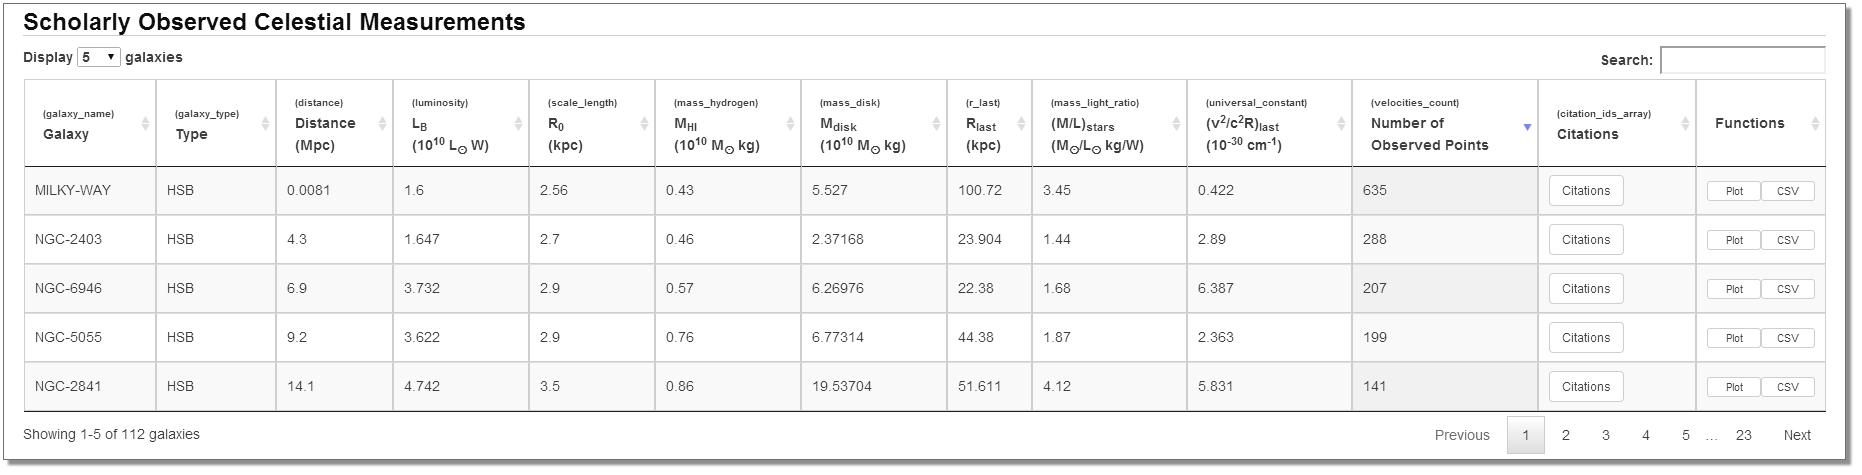
\includegraphics[width=\textwidth, height=2in, keepaspectratio]{socmtable}
\caption{The SOCM table where you can access all the galactic data.}
\label{socm_fig}
\end{figure*}


The idea is for astronomers to submit new measurements to the SOCM administrator (the authors) for approval. Thus creating a single means of distributing validated measurements of hundreds of galaxies. The input data can then be sent to RoCM. This way, if new galaxies get submitted and accepted, RoCM will always have the most up-to-date data that is provided. As an added feature, SOCM was created to also serve as a simple central database.  Thus, researchers may also pull from the SOCM application programming interface (API) to use the data for other applications other than rotation curve modeling.  When data and parameters are pulled from SOCM outside of RoCM, all of the proper units as well as citations are preserved.



\section{RoCM Functionality}

RoCM seeks to bring together the equations described above, and create a workstation for astrophysicists to quickly and easily model galaxies. The tool consists of 7 major components that all contribute to the powerful functionality we've provided in RoCM:
\begin{enumerate}
       \item The SOCM table drop down for easy access to the database (to select galaxies to plot or download).
       \item The rotation velocity over distance (Vel vs. R) graph to plot models against collected data.
       \item Parameter sliders to manipulate ALL values within galactic models (for parameter fitting purposes).
       \item A workstation for users to import custom parameters outside the ones already described.
        \item A way to visualize the simulation of the rotation curve (RoCS).
       \item A section for users to import their models in LaTeX format (for better understanding the behavior of parameters within each equation). 
       \item An option to export model graphs into .svg format.

\end{enumerate}



\subsection{Accessing the SOCM database from RoCM}
Figure \ref{socm_fig} shows the table of galactic data that is generated from the SOCM database. The user can sort by value, or search within the table to select a galaxy they would like to plot. The user can also download the parameter and velocity data of the galaxy in a CSV format.

--\textbf{TODO:} Talk about citations in the datebase. -- 
%The Milky Way data came from \cite{kundu} and \cite{sofue}. The rest of the data included in SOCM came from \cite{mannheim}. 


\subsection{Curve Plot for Rotation Velocity}

--\textbf{TODO: } Smooth out the 'Figure' references --

The main focus of RoCM is the curve plotting tool. Each galactic model is provided in the legend and can be displayed if clicked. The Milky Way's rotation curve can be seen in Figure \ref{milkywayplot}. To see a full screen-shot of the main RoCM page, see Figure \ref{rocm_fig}. You can see the $\chi^2$ table for each model %(Figure \ref{chi_fig})
 as well as a table of the current parameter values that can be directly edited via the input text box in Figure \ref{param_table_fig} or the parameter sliders drop down (shown in Figure \ref{slider_fig}). 

\begin{figure}[h!]
\centering
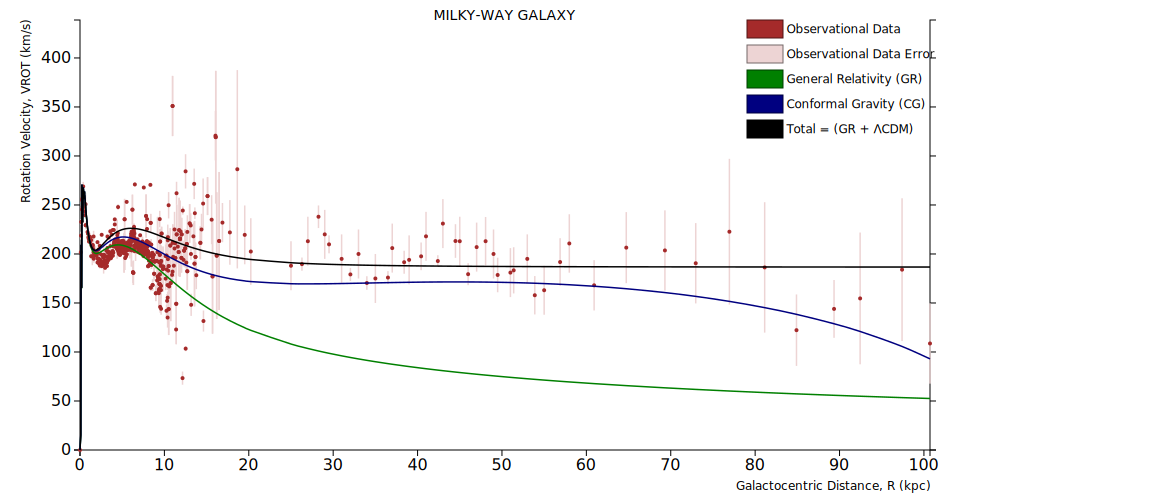
\includegraphics[width=\textwidth]{MILKY-WAY}
\caption{The plotted GR, CR, total $\Lambda CDM$ models over the observational data for the Milky Way (generated from RoCM).}
\label{milkywayplot}
\end{figure}

Having the $\chi^2$ value presented to the user shows the goodness of fit for each model. We implemented a $\chi^2$ variance because the observational data contains errors, $\mu$, and can be tested with
\begin{equation}
\chi^2 = \sum \frac{(O-E)^2}{\mu^2}
\end{equation} 
where $O$ is the observed data and $E$ is the experimental/model data. 

%\begin{figure}[h!]
%\centering
%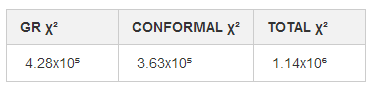
\includegraphics[width=2.5in]{MILKY-WAY-CHI2}
%\caption{The $\chi^2$ table for the Milky Way galaxy.}
%\label{chi_fig}
%\end{figure}
%
%\begin{figure}[h!]
%\centering
%\includegraphics[width=3.5in]{MILKY-WAY-PARAMS2}
%\caption{The mutable parameters table for the Milky Way galaxy.}
%\label{param_table_fig}
%\end{figure}

\begin{figure}[h!]
\centering
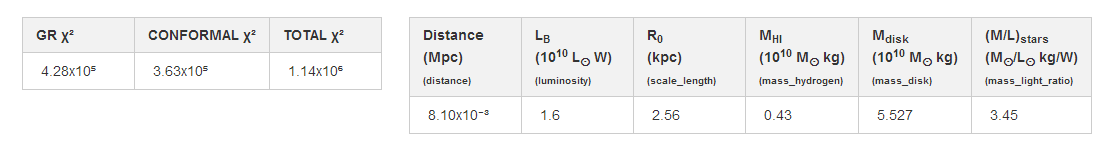
\includegraphics[width=\textwidth]{MILKY-WAY-CHI-PARAMS}
\caption{The $\chi^2$ table and mutable parameters table for the Milky Way galaxy.}
\label{param_table_fig}
\end{figure}

\subsection{Parameter Fitting Sliders}

The power of RoCM lies within these parameter sliders. The user can adjust the minimum and maximum of the parameters and slide the bar to see the how the changes effect the curves on the plot. This responsive visualization helps aid in understanding how each parameter behaves in the theories that use it.  Since the sliders are built into the workstation, one can see the effect they have on the enabled curves immediately.

\begin{figure}[h!]
\centering
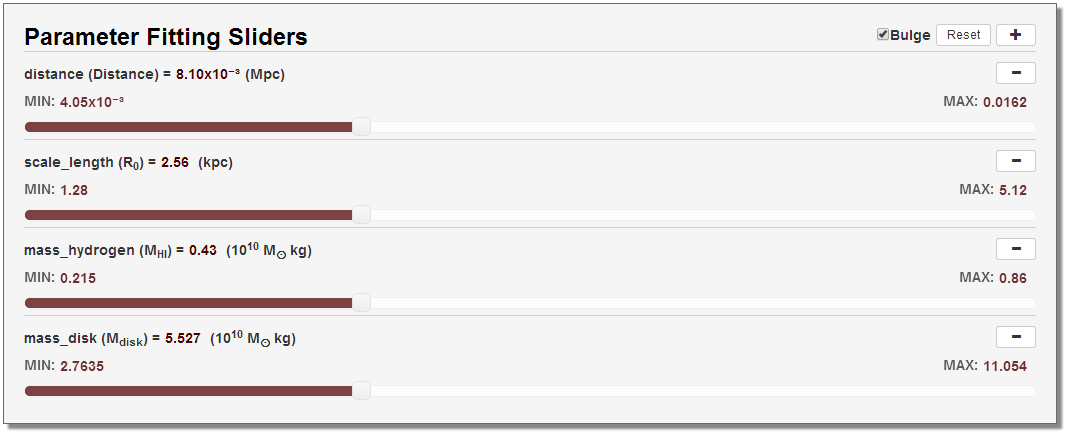
\includegraphics[width=0.8\textwidth]{paramslider_long}
\caption{Parameter fitting sliders with min and max values.}
\label{slider_fig}
\end{figure}


\subsection{User Defined Models and Parameters}
The discussed models, namely GR, $\Lambda CDM$, and CG aren't the only theories that model galaxies. Thus, users have the ability to write a model in JavaScript to import directly into RoCM. The User Defined Model workbench (Figure \ref{udm}) opens RoCM up for any and all models that want to be compared against each other. The function should be in the form:
\begin{center}
\begin{tabular}{c}
\begin{lstlisting}
function MODELNAME(R){
  var rotation_velocity;
  // The implemented JavaScript model
	
  return rotation_velocity; 
}
\end{lstlisting}
\end{tabular}
\end{center}

On the actual RoCM tool, user tutorials are provided to allow for quick input of the suggested models.  As RoCM grows in scope, we plan on having all of the major competing theories already input into the RoCM hard coding.


\subsection{Constants and Conversions}
Since it is the goal of RoCM to allow for any model, we must then also allow the user to manipulate some of the hard coding of RoCM as well.  Thus, constants can be changed if needed (see for example some alternative gravitational theories based on G not being constant). The contents can be retrieved and manipulated based on the following CONST commands. We also have provided some useful and common conversions hard coded into RoCM that can be accessed via the CONVERT commands.\begin{center}
\begin{tabular}{l !{\color{lightgray}\vrule} r}
\begin{lstlisting}
// Speed of light
CONST.get("c");
CONST.get("speed_of_light");

// Solar mass
CONST.get("Mo");
CONST.get("solar_mass");

// Solar luminosity
CONST.get("Lo");
CONST.get("solar_luminosity");

// Gravitational constant
CONST.get("G");
CONST.get("gravitational_constant");

// Schwarzschild radius
CONST.get("B*");
CONST.get("schwarzschild_radius");
\end{lstlisting}
&
\begin{lstlisting}
CONVERT.pc_to_kpc(pc)
CONVERT.Mpc_to_kpc(Mpc)
CONVERT.kpc_to_Mpc(kpc)
CONVERT.kpc_to_pc(kpc)
CONVERT.kpc_to_km(kpc)
CONVERT.km_to_kpc(km)
CONVERT.km_to_cm(km)
CONVERT.km_to_m(km)
CONVERT.cm_to_kpc(cm)
CONVERT.cm_to_km(cm)
// GeV/cm^3 to kg/km*s^2
CONVERT.GeVcm3_to_kgkms2(GeVcm3)
CONVERT.arcsec_to_degree(arcsec)
CONVERT.degree_to_arcsec(degree)
CONVERT.rad_to_deg(rad)
CONVERT.deg_to_rad(deg)
\end{lstlisting}
\end{tabular}
\end{center}


\subsection{Rotation Curve Simulation}

Although theorists in the field of gravity are quite fluent in rotation curve discussions, to an audience that has never been exposed to the rotation curve problem, their use and influence on the current paradigm may be elusive. RoCM has a built in function in the workstation to simulate and animate the current model in the workstation, The Rotation Curve Simulation (RoCS). The user can simulate either just the observational data, or a specified model against the data. The color scale represents the relative {\color[HTML]{EA051C} minimum} and {\color[HTML]{1AAF3A} maximum} velocity for the stars around the center of the galaxy. The scale helps recognize when the rotation curve simulation of a model doesn't match up with the observational data.



\begin{figure}[h!]
\centering
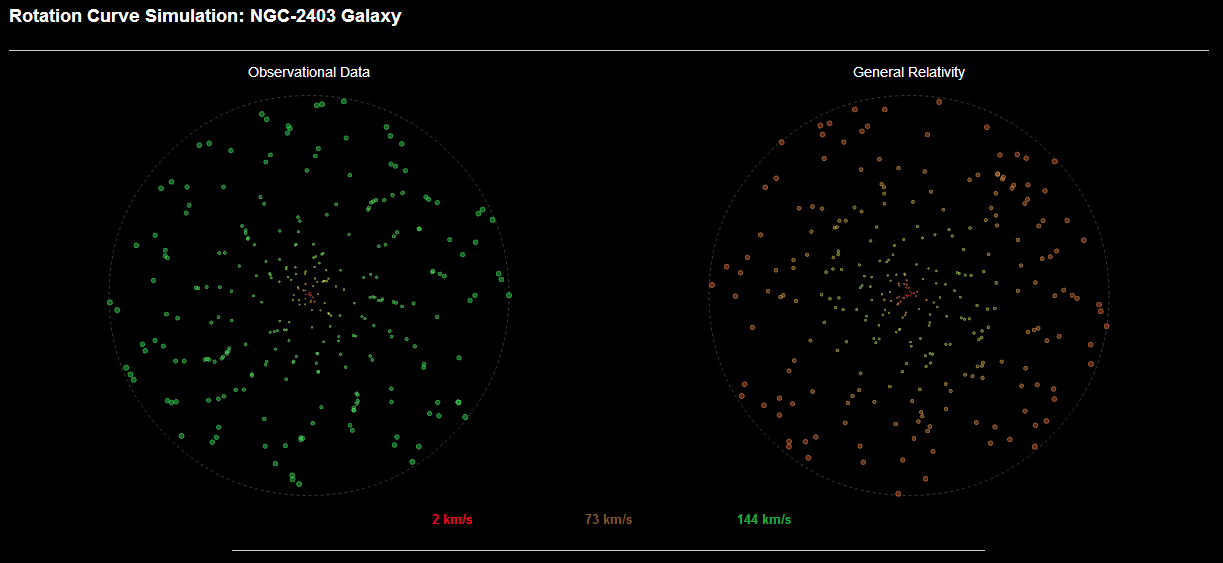
\includegraphics[width=0.9\textwidth]{NGC-2403-GR}
\caption{When viewing a model in RoCS side by side with the simulated observational data, it's clear to see where the velocity inconsistencies arise within the modeled galaxies. The biggest difference is when the data is compared to the GR prediction for NGC-2403. The inner parts of the galaxy seems to match the data. But about half way out, the velocity starts to slow down as described by the GR prediction, and the data stays uniform.}
\label{ngc2403gr}
\end{figure}


\begin{figure}[h!]
\centering
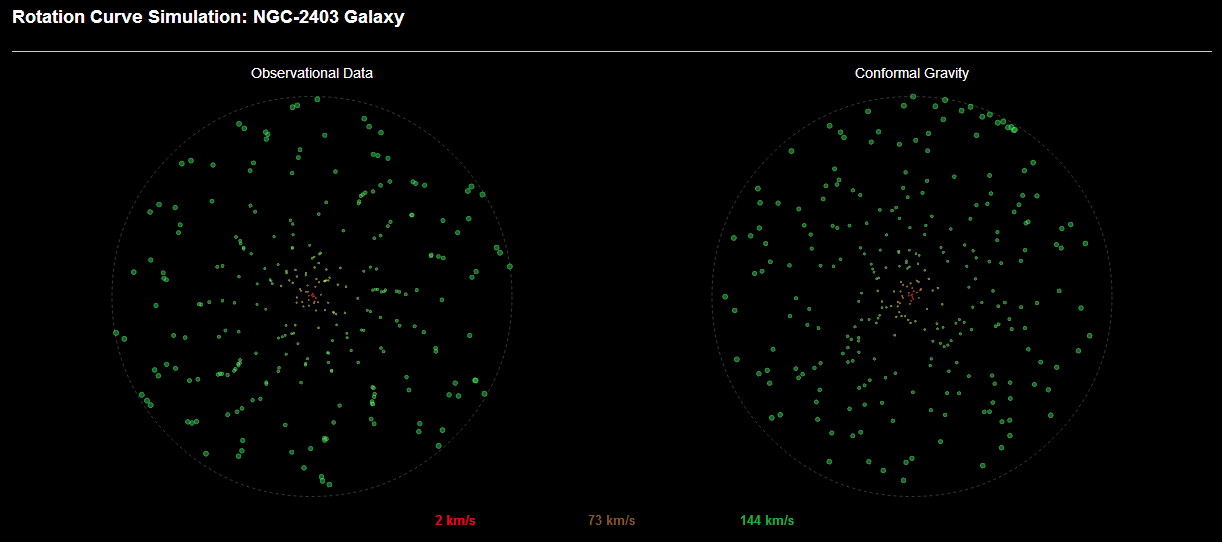
\includegraphics[width=0.9\textwidth]{NGC-2403-CG}
\caption{As an alternative, the CG prediction for NGC-2403 matches clearly with the observational data.}
\label{ngc2403cg}
\end{figure}


\begin{figure}[h!]
\centering
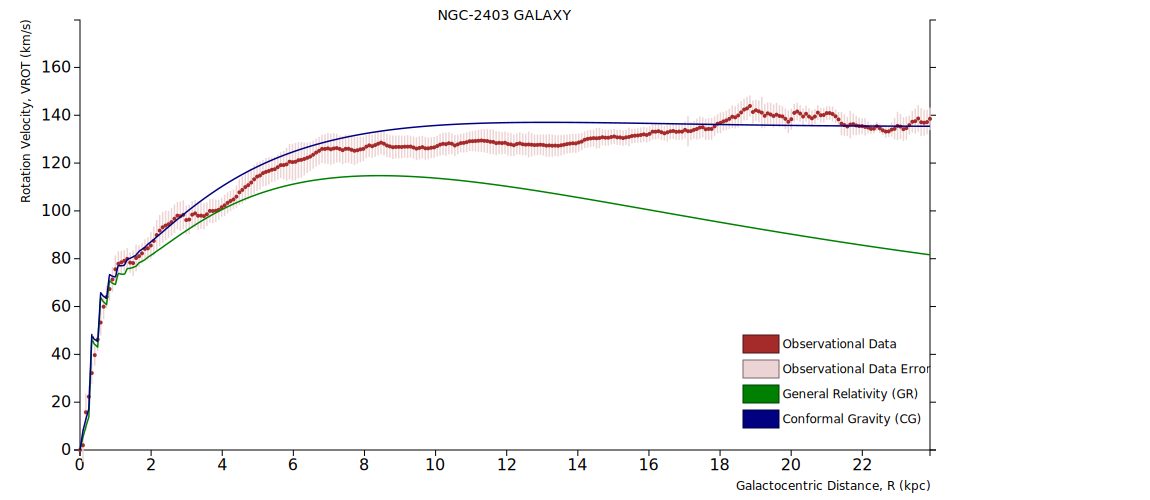
\includegraphics[width=\textwidth]{NGC-2403}
\caption{The NGC-2403 galaxy predicted with GR and CG plotted within RoCM shows that the GR curve starts to gradually decline as the CG curve stays consistent with the observational data. The parameters for each curve can be fitted to minimize the $\chi^2$ variance, all done through the parameter sliders functionality.}
\label{ngc2403plot}
\end{figure}


\newpage

\section{Conclusion}
The hope is that astronomers will use SOCM to upload observational data into one central location. Astrophysicists then can use RoCM to test that data against several galactic models to finally understand the dynamics of galaxies. 

	 We are pleased to announce that SOCM is open to the public at socm.herokuapp.com, where users can now view our database of collected measurements and developers may use our API endpoints to use in their own endeavors. RoCM is hosted online and can be found at www.wit.edu/rotationcurve. Each project individually is a contribution to the open source community and can be found here: https://github.com/RoCMSOCM.



\section*{Acknowledgment}

The authors would like to thank the departments of Sciences and Computer Science at WIT for allowing the work on RoCM and SoCM as a senior capstone project. J. G. O'Brien would like to thank Crystal Bailey, APS and SPS for the generous travel grant for R. J. Moss to present this work at APS April meeting 2014. The authors would also like to thank Chuck Hotchkiss for his continued support for undergraduate research projects at WIT, and for a matching travel grant for dissemination of this work. The authors would also like to thank Dr. Sophia Cizneros for her input into the creation of a useful database for theorists.

We would also like to thank Patrick McGee and David Miller for their help building the SOCM database. Alex Clement and Professor Mohammed Anwaruddin have also helped shape the outcome of the RoCM tool, so we thank them for their support.



\bibliographystyle{abbrv}
\bibliography{citations}

%\newpage
\hspace{\textwidth}

\section*{Appendix: Rotation Curve Modeler Screenshots}

\begin{figure*}[h!]
\centering
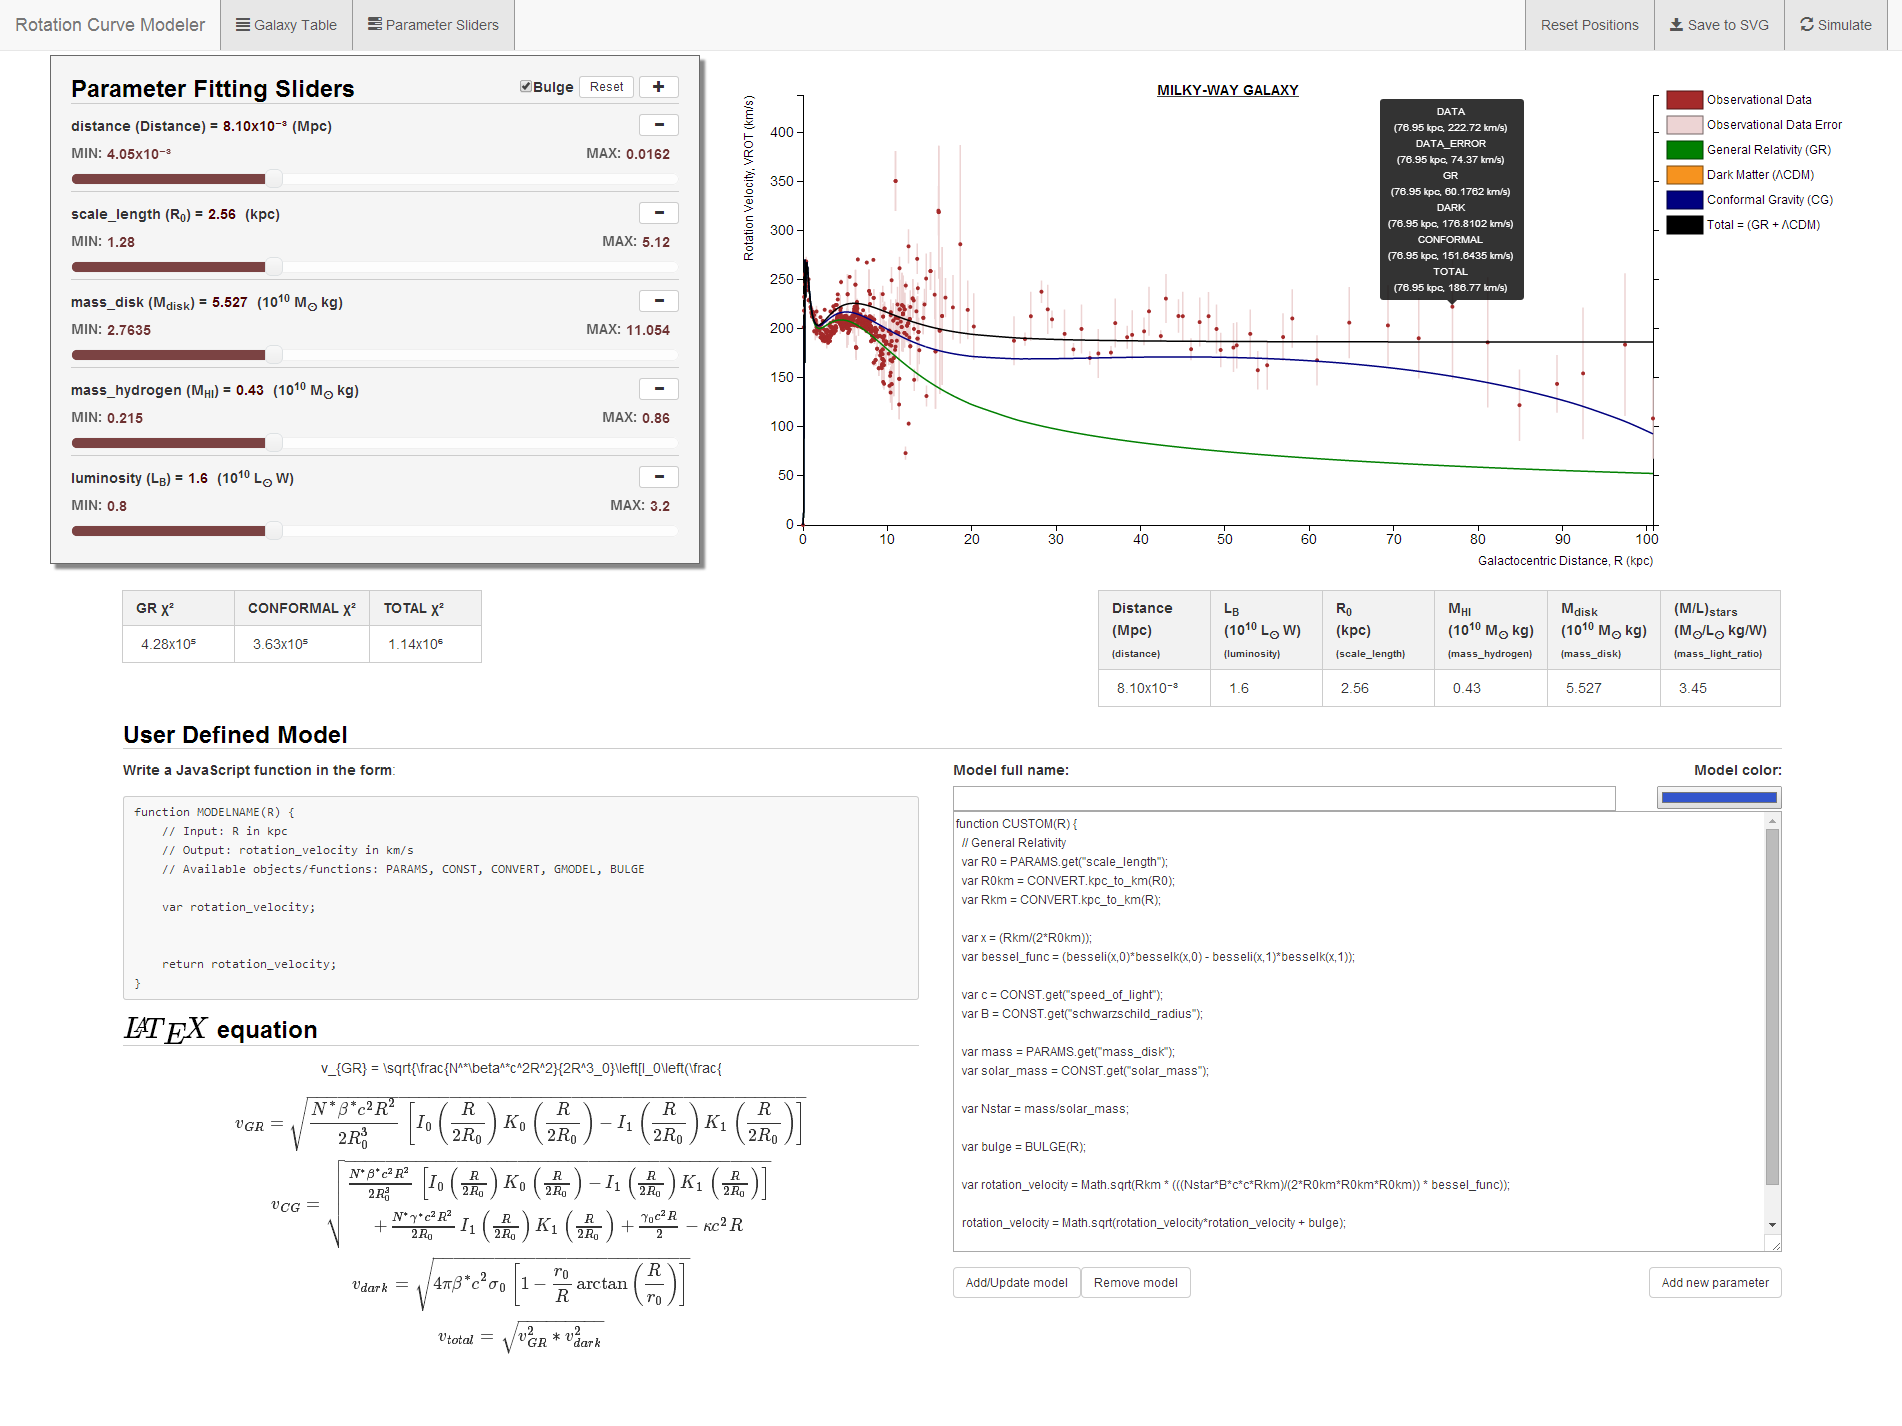
\includegraphics[width=\textwidth, frame, trim = -1cm -1cm -1cm -1cm, clip]{rocm_screenshot_full}
\caption{The main RoCM page where users can plot the specified galaxy (the Milky Way galaxy is shown). The User Defined Model workbench provides a way to import a JavaScript function to locally run additional models.}
\label{rocm_fig}
\end{figure*}



\end{document}